\section{Three frozen intervention mechanisms}
\label{sec:abc-mechanisms}
The new comparison changes mechanisms in the existing transient B model,
rather than selecting an easier service after seeing outcomes. All three
families and the eighteen formal identities are fixed before their new runs.
Each task has an immutable current input and one legal intervention. The service
requires one matching eight-byte application frame by 100 ms, valid independent
energy and receiver accounting, deduplication, and transient-voltage feasibility.
The 150 ms trajectory uses a 0.1 ms step. The evaluator is the same within each
task and across arms. Figure~\ref{fig:abc-mechanisms} reads the saved traces;
no new simulation is used to construct it~\cite{abcb,abcaudit}.

\begin{figure}[tbp]
\centering
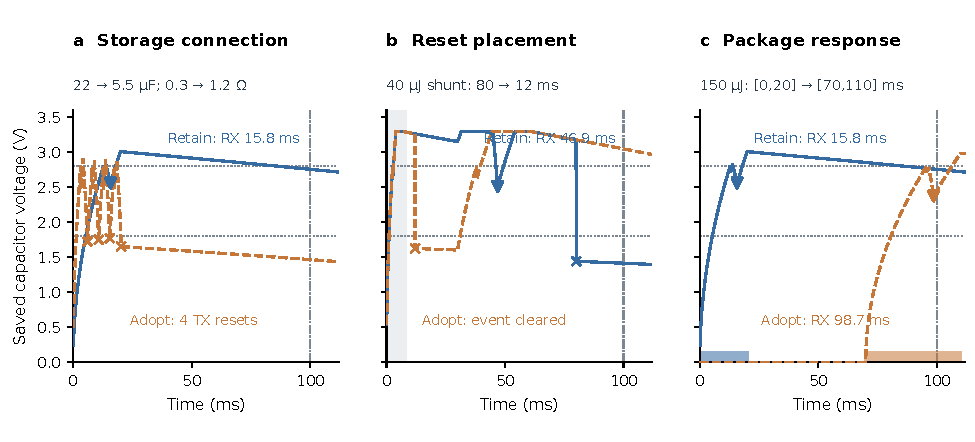
\includegraphics[width=\linewidth]{figures/mechanism-traces.pdf}
\caption{Frozen mechanism changes and saved post-step capacitor voltage.
Blue solid is retain; orange dashed is adopt. Triangles mark actual first
reception and crosses mark saved brownouts; dotted horizontal lines are the
2.8/1.8 V ready/off thresholds. The vertical dash-dot line is the 100 ms
deadline. (a) Series-equivalent storage produces four interrupted transmissions.
(b) Moving the shunt before TX clears volatile pending state; grey shading is
the eight-millisecond contact window. The retain reset is after delivery.
(c) Coloured strips mark prescribed source windows; the delayed intervention
still receives at 98.7 ms. These are five distinct digital exact inputs, with
the common retain trace reused in (a) and (c), not six physical experiments.}
\label{fig:abc-mechanisms}
\end{figure}

\subsection{Storage connection changes the buffer available to one transmission}
The storage family changes two identical ideal cells from parallel to series
while holding the PMIC clamp at 3.3 V. With per-cell capacitance $C_c=11~\mu$F
and ESR $R_c=0.6~\Omega$, the static equivalents are
\begin{equation}
 (C_{\parallel},R_{\parallel})=(2C_c,R_c/2),\qquad
 (C_{\rm series},R_{\rm series})=(C_c/2,2R_c).
\end{equation}
Thus capacitance changes from 22 to $5.5~\mu$F and ESR from 0.3 to
$1.2~\Omega$. The prescribed 7.5 mW source lasts 20 ms in both inputs;
the ideal passive event latch is unchanged. This mapping does not model cell
balancing, voltage-rating changes, leakage mismatch or package parasitics.

Retain receives at 15.8 ms. Adopt boots earlier, begins transmitting at 4.3 ms,
and resets at 6.1 ms before completing the two-millisecond frame. Four
transient resets occur by 20.2 ms and no valid frame arrives. Independent
energy conservation passes, while event reception and transient-voltage service
fail. Earlier readiness and adequate source integral are therefore insufficient
for this transaction. The stored energy above the off threshold, boot work,
ongoing harvest and loaded-rail guard jointly govern completion. A proxy that
compares only capacitor energy with TX work is not an exact failure theorem
when the source can replenish energy during TX.

\subsection{Reset placement changes event availability without changing its energy}
The reset family retains $10~\mu$F storage, a volatile event selector, a contact
from 0 to 8 ms, and earliest TX at 45 ms. Two source pulses supply
210~$\mu$J in total. The intervention moves the same 40~$\mu$J shunt
from 80 to 12 ms; it does not change its integral or insert another event.
Both trajectories first boot at 2.7 ms and capture the event during the contact.

Retain completes delivery at 46.9 ms, before its 80.1 ms reset. Adopt resets
at 12.1 ms, after contact has ended and before transmission is permitted.
Its volatile pending state is cleared. A second boot at 38.1 ms cannot recapture
an already ended contact; no frame is sent. Both independent energy and
receiver-integrity checks pass, but the intervention's event-reception
predicate fails. The discriminating object is the ordering of capture,
state-clearing reset and send, together with the actual reset semantics.
A post-delivery reset in retain does not demonstrate that volatile memory
preserves an undelivered event across reset.

\subsection{Package response changes usable time while preserving total input}
The package family transforms the prescribed rectangular source from
7.5 mW on $[0,20]$ ms to 3.75 mW on $[70,110]$ ms. Both provide
150~$\mu$J. Device parameters, event at zero, passive mechanical latch
and deadline are unchanged. The late input first boots at 95.8 ms and receives
at 98.7 ms, leaving 1.3 ms before the deadline; both retain and adopt pass.

This case is deliberately reported as a passing intervention. The shift does
not imply failure merely because it resembles a late pulse. Conversely, total
energy alone does not establish its tight reception margin. The passive latch
allows the event to remain available before electrical startup. The input
transformation is an assumed package-response law applied to the existing
port model; it is not a measured mechanical transfer function or a new
load-dependent source model. All family judgments remain digital and
physically uncalibrated~\cite{abcb}.
\FloatBarrier
